\documentclass[reqno,12pt,oneside]{report} % right-side equation numbering, 12 point font, print one-sided
%\documentclass[reqno,12pt,twoside,openright]{report} % right-side equation numbering, 12 point font, print two-sided, Chapters start on odd pages. Rackham only accepts one-sided, so this is for personal printings.

\usepackage{rac}         % Use Rackham thesis style file
%\usepackage{aas_macros}  % To allow the reading of ADS journal references in the bibliography
\usepackage[intlimits]{amsmath} % Puts the limits of integrals on top and bottom
\usepackage{amsxtra}     % Use various AMS packages


\usepackage{tabularx} % Required for the tabularx environment
\usepackage{ragged2e} % For justified text in cells
\usepackage{listings}
\usepackage{minted}
\usepackage{underscore}
\usepackage{placeins}
\usepackage{float}


\usepackage{amsthm}
\usepackage{amssymb}
\usepackage{graphicx}    % Add some packages for figures. Read epslatex.pdf on ctan.tug.org

\usepackage{rotating}
\usepackage{color}
\usepackage{xspace}
\usepackage{mdframed}
\usepackage{epsfig}
\usepackage{subfigure}   % To make subfigures. Read subfigure.pdf on ctan.tug.org
\usepackage{multirow}

\usepackage{verbatim}
\usepackage[numbers]{natbib}      % Allows you to use BibTeX
\usepackage{acronym} % For the List of Abbreviations. Read acronym.pdf on ctan.tug.org
\usepackage{booktabs}% http://ctan.org/pkg/booktabs
\newcommand{\tabitem}{~~\llap{\textbullet}~~}
\usepackage{indentfirst}
\usepackage{enumitem}
\usepackage{setspace}
\usepackage[T1]{fontenc}
\usepackage[utf8]{inputenc}
%\usepackage[options ]{algorithm2e}
\usepackage{algpseudocode}
\usepackage{ifthen}
%\usepackage{mathptmx} 
%\usepackage[acronym]{glossaries}
%\usepackage{nomencl}
%\usepackage[noend]{algpseudocode}
%\usepackage[linesnumbered,ruled,vlined]{algorithm2e}

\usepackage[intoc]{nomencl}
\usepackage{tikz}
\usetikzlibrary{shapes.geometric, arrows}

\usepackage{url}
%\usepackage{breakurl}
%\usepackage[breaklinks]{hyperref}
% \usepackage{hyperref}
 
 \usepackage{algorithm,algpseudocode}


%\usepackage[latin1]{inputenc}
%\usetikzlibrary{shapes,arrows}
\tikzstyle{startstop} = [rectangle, rounded corners, minimum width=3cm, minimum height=1cm,text centered, draw=black, fill=red!30]
\tikzstyle{io} = [trapezium, trapezium left angle=70, trapezium right angle=110, minimum width=3cm, minimum height=1cm, text centered, draw=black, fill=blue!30]
\tikzstyle{process} = [rectangle, minimum width=3cm, minimum height=1cm, text centered, draw=black, fill=orange!30]
\tikzstyle{decision} = [diamond, minimum width=3cm, minimum height=1cm, text centered, draw=black, fill=green!30]
\tikzstyle{arrow} = [thick,->,>=stealth]

%%%<


\usepackage[nottoc,notlof,notlot]{tocbibind}
\renewcommand\bibname{References}

\makenomenclature
%\makenomenclature
  % Allows you to specify the line spacing
%\doublespacing
\onehalfspacing %for 1.5 spacing, %\doublespacing for 2.0 spacing.
\newcommand{\sun}{\ensuremath{\odot}} % sun symbol is \sun
%%%%%%%%%%%%%%%%%%%%%%%%%%%%%%%%%%%%%%%%%%%%%%%%%%%%%%%%%%%%%%%%%%%%%%%%%%%%%%%

% Various theorem environments. All of the following have the same numbering
% system as theorem.

\theoremstyle{plain}
\newtheorem{theorem}{Theorem}
\newtheorem{prop}[theorem]{Proposition}
\newtheorem{corollary}[theorem]{Corollary}
\newtheorem{lemma}[theorem]{Lemma}
\newtheorem{question}[theorem]{Question}
\newtheorem{conjecture}[theorem]{Conjecture}
\newtheorem{assumption}[theorem]{Assumption}

\theoremstyle{definition}
\newtheorem{definition}[theorem]{Definition}
\newtheorem{notation}[theorem]{Notation}
\newtheorem{condition}[theorem]{Condition}
\newtheorem{example}[theorem]{Example}
\newtheorem{introduction}[theorem]{Introduction}

\theoremstyle{remark}
\newtheorem{remark}[theorem]{Remark}
%%%%%%%%%%%%%%%%%%%%%%%%%%%%%%%%%%%%%%%%%%%%%%%%%%%%%%%%%%%%%%%%%%%%%%%%%%%%%%%

\numberwithin{theorem}{chapter}     % Numbers theorems "x.y" where x
                                    % is the section number, y is the
                                    % theorem number

%\renewcommand{\thetheorem}{\arabic{chapter}.\arabic{theorem}}

%\makeatletter                      % This sequence of commands will
%\let\c@equation\c@theorem          % incorporate equation numbering
%\makeatother                       % into the theorem numbering scheme

%\renewcommand{\theenumi}{(\roman{enumi})}

%%%%%%%%%%%%%%%%%%%%%%%%%%%%%%%%%%%%%%%%%%%%%%%%%%%%%%%%%%%%%%%%%%%%%%%%%%%%%%

% If printing two-sided, this makes sure that any blank page at the
% end of a chapter will not have a page number.
\makeatletter
\def\cleardoublepage{\clearpage\if@twoside \ifodd\c@page\else
\hbox{}
\thispagestyle{empty}
\newpage
\if@twocolumn\hbox{}\newpage\fi\fi\fi}
\makeatother

%%%%%%%%%%%%%%%%%%%%%%%%%%%%%%%%%%%%%%%%%%%%%%%%%%%%%%%%%%%%%%%%%%%%%%%%%%%%%%

%This command creates a box marked ``To Do'' around text.
%To use type \todo{  insert text here  }.

\newcommand{\todo}[1]{\vspace{5 mm}\par \noindent
\marginpar{\textsc{To Do}}
\framebox{\begin{minipage}[c]{0.95 \textwidth}
\tt\begin{center} #1 \end{center}\end{minipage}}\vspace{5 mm}\par}



\begin{document}
%\bibliographystyle{ieeetr}
%\bibliographystyle{plain}    % Set the bibliography style. agu04, plain, alpha, etc.
% Title page as required by Rackham dissertation guidelines
\titlepage{A Voice-Controlled Web Navigation System}{ 212126}{Professional Masters in Information Technology}
{Information Technology}{October 2025}
{Professor Shamim Al Mamun, PhD}

% Begin the front matter as required by Rackham dissertation guidelines
\initializefrontsections

% Optional Frontispiece
%\frontispiece{\includegraphics[width=6in]{Intro/Happy} Find a cool picture to go here.}

% Optional, but recommended, Copyright page
%\copyrightpage{Your Name}

% Page numbering. If you don't include a frontispiece or copyright page, you'll need to change this for two-sided printing.
\makeatletter
\if@twoside \setcounter{page}{4} \else \setcounter{page}{1} \fi
\makeatother

% Optional Dedication page
%\dedicationpage{To Our Beloved Parents}


%Optional declaration page
\startdeclarationpage
We hereby declare that this thesis is based on the results found by ourselves. Materials
of work found by other researcher are mentioned by reference. This thesis, neither in
whole nor in part, has been previously submitted for any degree.

\bigskip
\bigskip
\bigskip


\begin{tabular}{p{5cm}p{5cm}p{5cm}}
\centering
  % after \\: \hline or \cline{col1-col2} \cline{col3-col4} ...
     &  &   \\
     &  &   \\
     &  &   \\
  \rule{3.5cm}{1pt} & \rule{3.5cm}{1pt} & \rule{3.5cm}{1pt}\\
  XXXX & YYYY  &ZZZZ\\
  Roll:xxxx & Roll:yyyy  &Roll:yyyy\\

\end{tabular}

\label{declaration}


%Optional Certificate page
\startcertificatepage
The project titled “A Voice-Controlled Web Navigation System” submitted by Sudipta Sarker, ID: 212126, Session: Summer 2021, has been accepted as satisfactory in partial fulfillment of the requirement for the degree of Professional Masters in Information Technology on the 11th of October 2025.

%\bigskip

\bigskip
\bigskip
\bigskip

\noindent \begin{tabular}{l}

  % after \\: \hline or \cline{col1-col2} \cline{col3-col4} ...
  \rule{4cm}{1pt} \\
  Professor Shamim Al Mamun, PhD\\ % replace it
  Supervisor\\

\end{tabular}


%Accepted and approved in partial fulfilment of the requirement for the degree Professional Master in Information Technology.


\begin{center}
   \textbf{BOARD OF EXAMINERS}
\end{center}
\noindent \begin{tabular}{lp{1cm}r}
\centering
  % after \\: \hline or \cline{col1-col2} \cline{col3-col4} ...
  \rule{4cm}{1pt}&\\
     Dr. M. Shamim Kaiser  && Coordinator  \\
     Professor, IIT, JU  & & PMIT Coordination Committee  \\
     & &  \\
     \rule{4cm}{1pt}&\\
    Dr. Risala Tasin Khan  & &  Member, PMIT Coordination Committee   \\
     Professor, IIT, JU  & &\& Director, IIT\\
    & &  \\
     \rule{4cm}{1pt}&\\
     Dr. Jesmin Akhter & & Member  \\
      Professor, IIT, JU  & & PMIT Coordination Committee  \\
     &  \\
     \rule{4cm}{1pt}&\\
     K M Akkas Ali   & & Member  \\
      Professor, IIT, JU  & & PMIT Coordination Committee  \\
      &  \\
     \rule{4cm}{1pt}&\\
      Dr. Rashed Mazumder & &  Member  \\
      Associate Professor, IIT, JU  & & PMIT Coordination Committee  \\
     
  %\rule{4cm}{1pt} & \rule{4cm}{1pt} & \rule{4cm}{1pt}\\
   

\end{tabular}


%\noindent \begin{tabular}{p{5cm}p{4cm}p{5cm}}
%\centering
  % after \\: \hline or \cline{col1-col2} %\cline{col3-col4} ...
   %  &  &   \\
    % &  &   \\
     %&  &   \\
  %\rule{4cm}{1pt} &  & \rule{3.5cm}{1pt}\\
  %Jesmin Akhter &   &K M Akkas Ali\\
  %Chairman &   &Member\\
   %  &  &   \\
    % &  &   \\
  %\rule{3.5cm}{1pt}& & \rule{3.5cm}{1pt}\\
   %Shamim Al Mamun&   &Prof. Dr. M. A. Mottalib \\
  %Member &   &Member (External) \\
%\end{tabular}


\label{Certificate}



% Optional Acknowledgements page
\startacknowledgementspage
	
	At first, I bow my head in gratitude to the Almighty God for granting me strength and blessings to complete this project. Without his guidance it was not possible to complete this journey successfully.
	
	I would like to express my heartfelt appreciation and gratitude to my respected supervisor, Professor Dr. Shamim Al Mamun, whose support, valuable guidance and constructive feedback played an important role to achieve this goal. His motivation and guidance kept me focused and straight forward to implement this project from the scratch to the end.
	
	
	
	My deepest respect and thanks to the Director and the honorable faculty members of the Faculty of PMIT, Jahangirnagar University for providing me with necessary academic facilities and inspiration during my study period. Their dedicated teaching and cooperative attitude helped me to enhance my knowledge and gain innovative ideas such as this project.
	
	Finally I would like to express my gratitude to my friends, classmates and others who directly or indirectly helped me in completing this project. I am also thankful to the administrative and staffs of PMIT for their cooperation and accurate information whenever required.
	
	
\label{Acknowledgements}

%Optional Abstract page
\startabstractpage

		This project focuses on the development of a Chrome extension controlled by voice to improve user interactivity with web browser. Voice based browsing extensions are explored in the modern era, but most of them are limited to certain languages or do not provide flexible tab control, inline search or smooth speech interaction. The proposed solution introduces a lightweight browser extension which supports both Bangla and English commands and provides flexible features like switching between tabs, inline search for Google and Wikipedia, fill up forms, read out selected text through speech. To achieve this, we implemented speech recognition APIs, intent-based command matching and parsing for accurate result with modular Javascript arhitechture for scalability. Chrome extension APIs were integrated here for tab management, content handling and background propagation. The system was test through real browser scenerio and successfully performed site navigation, click through expected links, inline search with dual languages without noticeable lag. A special feature is added for auto silence detection and highlight-based read-0out functionality by integrating speech recognition APIs. The findings shows that the extension can help to reduce manual browsing effort by providing solutions for users with limited typing skills and handicuffs. This project shows that voice driven solution can improve web accessibility and multilingual abilities.
		
		\vspace{8pt}
		\textbf{Keywords}: Chrome extension, Speech recognition, APIs, Voice driven solution, Inline search.

	








































\label{Abstract}




% List of Abbreviation

\listofabbreviations % Optional. Abbreviations should be stored in a file named abbr.tex
% Optional in-dissertation Abstract Page
%\startabstractpage
%{The Title of Your Dissertation}{Your Name}{Chair: Albert Einstein}
%
		This project focuses on the development of a Chrome extension controlled by voice to improve user interactivity with web browser. Voice based browsing extensions are explored in the modern era, but most of them are limited to certain languages or do not provide flexible tab control, inline search or smooth speech interaction. The proposed solution introduces a lightweight browser extension which supports both Bangla and English commands and provides flexible features like switching between tabs, inline search for Google and Wikipedia, fill up forms, read out selected text through speech. To achieve this, we implemented speech recognition APIs, intent-based command matching and parsing for accurate result with modular Javascript arhitechture for scalability. Chrome extension APIs were integrated here for tab management, content handling and background propagation. The system was test through real browser scenerio and successfully performed site navigation, click through expected links, inline search with dual languages without noticeable lag. A special feature is added for auto silence detection and highlight-based read-0out functionality by integrating speech recognition APIs. The findings shows that the extension can help to reduce manual browsing effort by providing solutions for users with limited typing skills and handicuffs. This project shows that voice driven solution can improve web accessibility and multilingual abilities.
		
		\vspace{8pt}
		\textbf{Keywords}: Chrome extension, Speech recognition, APIs, Voice driven solution, Inline search.

	








































%\label{Abstract}

\section*{
\begin{center}
  LIST OF ABBREVIATIONS
\end{center}
}

\begin{tabular}{p{2.5cm}p{10cm}}
%\textbf{\symbab}  & \symbac\\
\textbf{IIT}  & Institute of Information Technology\\
\textbf{JU}  & Jahangirnagar University \\
\textbf{PMIT}  & Professional Masters in Information Technology \\
\textbf{API} & Application Programming Interface \\
\textbf{TTS} & Text to Speech


\end{tabular}



% List of Notatoin
% \listofnotations
% \section*{
% \begin{center}
%  LIST OF NOTATIONS
% \end{center}
% }
%




%\input{Preface}
%\label{Preface}
% Table of contents, list of figures, etc.
\listoffigures   % Required if there is more than one figure
\listoftables        % Required if there is more than one table
\tableofcontents     % Required

%\startprefacepage
\printnomenclature[1.5cm]

%%%%%%%%%%%%%%%%%%%\printnomenclature
%\clearpage



%\renewcommand{\arraystretch}{1.70}
%\begin{tabular}{p{2.5cm}p{10cm}}
%\centering
  %\rule{3.5cm}{1pt} & \rule{3.5cm}{1pt} & \rule{3.5cm}{1pt}\\
%  $\alpha$ & Define Alpha\\
%$\symba $ & \symbb\\
%$\symbc $ & \symbd\\
%$\symbe $ & \symbf\\
%$\symbg $ & \symbh\\
%$\symbi $ & \symbj\\
%$\symbk $ & \symbl\\
%$\symbm $ & \symbn\\
%$\symbo $ & \symbp\\
%$\symbq $ & \symbr\\
%$\symbs $ & \symbt\\
%$\symbu $ & \symbv\\
%$\symbw $ & \symbx\\
%\end{tabular}
%\newpage
%\begin{tabular}{p{2.5cm}p{10cm}}









%\listofmaps          % Required if there is more than one map
%\listofappendices    % Required if there is more than one appendix
%%%%--------------------------------------------------------------------------------
\startthechapters
% The individual files for each of the chapters are put here.
% Save each chapter of your thesis to a seperate tex file
% and then use the \input command to include this file in your
% thesis.  For instance you can save a file to "intro.tex" and
% then type \input{intro}.

 %\chapter{Introduction}
 \label{chap:Intro}
 


	\chapter{Introduction}
	\section{Overview}
	The rapid growth of the Internet makes the web browser an essential tool for various use cases like accessing information, analysis, performing tasks globally. Traditionally, users use web browser by using keyboards or using mice. This can be time consuming, boring, inconvenience and challenging for people who has limited typing skills or disabilities. Voice based technologies supported by speech recognition and natural language processing bring a ground-breaking change in this area by providing more accessible method of interacting with digital systems.
	
	
	This project focuses on the design and development of the voice controlled Chrome extension which supports Bangla and English. This extension allow users to search online from google and wikipedia, read selected text, can click the highlighted links and many more – all through voice commands. By enabling multiple language, the system enhances the usability to the people in Bangladesh where English is not the the primary language.
	
	
	\section{Limitation of Existing Works}
	Existing voice assistant solutions like Siri or Google Assistant are mostly designed for mobile devices or standalone device with limited integration with desktop browsers. Besides these systems are mostly English centric and lack of usability in Bangla language in some cases. 
	
	
	On the other hand, the existing browser extensions which support voice commands, very few of them integrate features like tab control, form fill up, click highlighted links, read selected text, click important links or inline search. Some of them consume more resources which make them  heavy-weighted browser uses. Very view extensions provide multilingual solutions that support both Banlga and English. So, these limitations motivated me to develop a dedicated browser extension which supports these features with multilingual inclusive.
	
	
	\section{Motivation}
	The motivation for this project grows inside me for the demand of more accessible and efficient browsing methods  for users who performs more multi tasks, need to write long queries, face difficulties to find a particular link in a who page. Similarly, some people has physical difficulties or find interest to listen text content rather than reading whole content. This browser extension with multilingual facilities can bridge this gaps making browsing faster and interesting by providing a lots of features. 
	
	\section{Problem Statements}
	Although the availability of the advanced voice assistant like Siri or
	Google Assistant, there is no lightweight Chrome extension that provides dual-language (English and Bangla) voice control with additional browsing facilities. Users currently lack the ability to:
	\begin{itemize}
		\item	Perform inline search through Google, Wikipedia or YouTube by voice.
		\item	Switch between specific browser tabs using voice recognition.
		\item   Control Media element interaction by voice.
		\item	Click highlighted links to navigate and find the expected links easily.
		\item	Fill up forms, listen the selected text.
	\end{itemize}
	
	This project addresses these issues by proposing and developing a proper voice based Chrome browser extension by including these features with multilingual support in Bangla and English.
	
	
	\section{Objectives}
	The main objectives of this research are:
	\begin{itemize}
		\item To design and develop a voice-based Chrome extension that allows users to interact with the web browser through natural speech commands.
		\item To support multilingual interaction (English and Bengali) so that both local and international users can easily interact with the browser.
		\item To perform different activities through browser like searching content on Google, Wikipedia, form filling, media control(play/pause/mute), click highlighted links etc. using voice commands.
	\end{itemize}
	\section{Research Outline}
	This project is structured into five major chapters:
	\begin{itemize}
		\item	Chapter 1 – Introduction: Provides the background, problem statement, motivation, objectives of the study and research outline.
		\item	Chapter 2 – Literature Review: Discusses about the existing solutions or related works, their features and limitations.
		\item	Chapter 3 – Proposed System Architecture: Explains the architecture, tools, speech recognition techniques and algorithmic approach to achieve the intended functionalities.
		\item	Chapter 4 – Implementation and Results: Describes coding modules, functionalities tested and the experimental outcomes.
		\item	Chapter 5 – Conclusion and Future Works: Summarizes the findings of the project, implications and some important improvements for future.
	\end{itemize}
	
	\section{Conclusion}
	In this chapter, background and motivation of the project are presented along with limitations of the existing solutions. Besides the problem statements and the objectives clearly dictate the necessity of the multilingual voice based Chrome extension. This chapter also provides the research outline which will guide the overall project design and implementation throughout the project. The next chapter will provide the review for the existing solutions and related works to identify the existing gaps which establish the foundation of the proposed system.
	






% \chapter{Literature Survey}
 
\chapter{Literature Review}
	\label{chapter:2}
	\section{Overview}
	Before initiating the development of the proposed voice controlled chrome extension, a detail study was conducted based on related existing tools, research works, extensions. This study gives a proper insight which helped to build this project. The study demonstrates the features of the existing works and review them about their limitations. It highlighted how this tools approached to implement voice recognition, natural language understanding and how to interact with the browser which forms the foundation for developing a enhanced proper voice controlled chrome extension with extensive features.
	
	The study also shows the importance of the response time, performance, user experience, supported languages of those works, By studying these works and papers, the opportunities of new features/solution have been identified.
	
	\section{Related Works}
	
	\subsection{Browser-based Voice Extensions}
	\textbf{Handsfree for Web \cite{handsfree}} provides a lots of set features including web search(Google, Wikipedia), click links, scrolling, form filling, media control, text reading and some basic browser control features. The strength of this system lie in extensive features and multilingual support(4 languages). But it has no integration with Gmail, Google Docs, or map related features.
	
	\textbf{Readme – TTS \cite{readme}} mainly focuses on the accessibilty of the browser supported by over 50 languages. It helps user to listen to text from webpage, emails and PDF. But this extension does not support browser control or media control. The limitation of this extension is less features, mainly focuses on text-speech features rather than browser interaction.
	
	\textbf{Hey Buddy – Chrome Voice Assistant\cite{heybuddy}} provides features for basic browsing interaction and media control including search, scrolling and link navigation. It is lightweight and easy to use but it does not support Bangla and does not provide some advanced features like email management and Google Doc interaction or custom commands.
	
	\textbf{LipSurf - Voice Control for the Web\cite{lipsurf}} allows user to interact with browser using voice commands. It supports tab control, form filling and media control. It provides a good set of features but does not integrate Bangla language to communicate.
    
	\textbf{Voice Typing\cite{voicetyping}} enables users to write text based on voice input. It receives voice input from users and translates it into text by using text-to-speech API. It does not come with other features like browser control or media control. Its scope is limited to type text only.
	
	\textbf{Speech Recognition Anywhere\cite{speechrec}} offers flexible features with multiple language support. It allows features to copy, paste and basic form filling. It supports browser control features but does not include advanced productivity tools. 
	
	Other notable extensions include: 
	\begin{itemize}
		\item	Text-to-Speech that Brings Productivity\cite{texttospeechprod} – TTS focused with limited control features.
		\item	Voice In Voice Typing\cite{voicein} – Dictation tool can be used for fill in forms and email writing specially.
		\item	Dictation for Gmail\cite{dictationgmail} – Specialized for email accessibility. 
		\item	Talkie: Text-to-Speech\cite{talkie} – Multilingual reading tool for selected text.
		\item	NaviVoice: Voice Input Productivity Assistant\cite{navivoice} – Limited browsing and form filling features are offered by this extension.
		\item	Voice Actions for Chrome (beta)\cite{voiceactions} – Simple browser commands(only able to search through query)
		\item	Say Play\cite{sayplay} – Media playback control. This extension is only used to control media content.
		\item	Neo\cite{neo} – Lightweight browsing and limited productivity features. Google searching by opening new site is feature here.
		\item	Speech to Text (Voice Recognition)\cite{speechtext} – Dictation focused.
		\item	Capti Voice\cite{captivoice} – Accessibility tool for reading and highlighting text.
		\item	Voice Control for Video\cite{voicecontrolvideo} – Media control only.
		\item	VCAT\cite{vcat} – Basic voice commands and limited browsing control.
		\item	Natural Reader Text to Speech\cite{naturalreader} – Multilingual reader for web pages, PDFs, emails.
		
        From the above discussion it is proved that no single extension currently offers browsing control, media control and multilingual accessibility(specially for Bangla) as an unit.
		
	\end{itemize}
	\subsection{Research-based Voice Systems And Academic Works}
	There are several academic and large-scale solutions provide detail insight fro voice-based systems rather than browser extensions.
	
	\textbf{Google Voice Access\cite{googlevoice}} offers accessibility, allow uses to navigate and control the system. While this system is highly effective for mobile devices but it does direct support desktop chrome browsing. Amazon Alexa Browser Integrations\cite{amazonvoice} allow users to do basic search and other tasks but it has dependency on the cloud services and limited to the devices.
	
	\textbf{A Voice Controlled E-commerce Web App\cite{voicecommerce}} focuses on the accessibility of online shopping tasks can be improved through voice commands. It presents that by using voice commands users can perform their shopping from e-commerce site smoothly and efficiently. But this paper does not present any interaction for browser accessibility through voice commands.
	
	Studies on \textbf{Voice-Based HCI\cite{researchstudies}} emphasized different parameters  which are critical for browser-based extension such as  response time, noise handling, and context recognition.
	
	\textbf{Accessibility research\cite{accessibilitystudies}} highlights the necessity of multilingual support, highlighting words during text to speech, and provides integration with different productivity tools.
	
	\textbf{Këpuska \& Bohouta (2017)\cite{kepuska2017comparing}} studied and compared  modern speech recognition APIs (Google, Microsoft, IBM Watson, CMU Sphinx) and referred that cloud-based systems achieve high accuracy while local engines allow offline processing.
	
	\section{Analysis of Findings}
	The analysis of reviewed extensions and academic systems shows that most browser based web extensions offers several features like basic navigation, read selected text, media control, some provides multilingual support but lack of integration with productivity applications. But as an unified system no extension can offer all the features with high response time and support voice commands for Bangla. 
	
	Research studies how accuracy, latency, noise handling, multilingual support with proper design can enhance the productivity of a voice-based solutions which builds the foundation for the proposed system.
	
	\section{Conclusion}
	In summary, the literature review shows that while there exists several extensions which provide partial voice-based browsing control, media control or TTS functionality, no solution offer an unified integrated solution by combining all important features and support for Bangla language. Existing academic research highlights the importance of accuracy, speed, and usability and latency, which are essential to incorporate into the design of the proposed system. The goal of the proposed extension is to bridge these gaps, providing a user-friendly, feature oriented, multilingual, and productivity based voice assistant tool for Chrome web browser.
	










%\chapter{System Model}
 \chapter{Proposed System Architecture}
\section{Introduction}
This chapter represents the methodology used in the development of the Voice Search Chrome Extension. The chapter focuses on the design, workflow and the core functionalities of the proposed system. This system enables users to control the browser for several facilities like search in the internet, form fill up, read the selected content and click the highlighted links through voice commands.

The methodology demonstrates modularity, scalability and user-friendliness. This system is divided into different logical components to ensure the accurate speech recognition and identify the correct command by parsing and executing the right operation. This chapter describes the architecture, workflow and features through diagrams, flowcharts and algorithm to make it easy to understand the system properly.

\section{System Architecture}
\section*{Overview of Components}
\begin{itemize} 
\item \textbf{User Interface Module:} Provides a floating microphone button for capturing voice input.
\item \textbf{Speech Recognition Module:} Converts spoken words into text using the browser’s Web Speech API.
\item \textbf{Command Processing Module:} Detects the language and identifies the user’s intent by matching text with predefined commands stored in JSON files (en.json, bn.json).
\item \textbf{Action Execution Module:} Performs the requested browser actions, including tab control, scrolling, inline search, media handling, link clicking, and form filling.
\item \textbf{Feedback Module:} Provides visual or audio feedback to the user, such as highlighting text during read-aloud or confirming executed actions.
\end{itemize}

\begin{figure}[H]
   \centering
   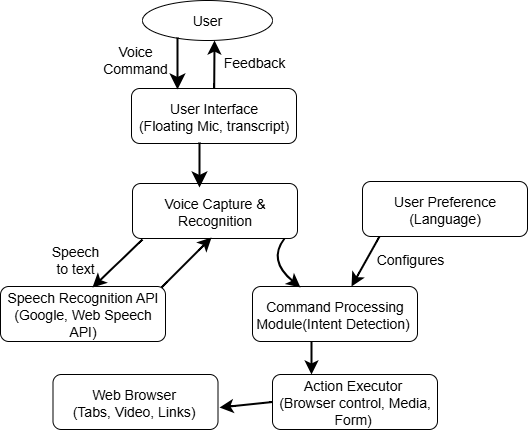
\includegraphics[width=4in]{latex/Chap3/system_architecture.png}
   \caption{Architecture of the Voice Search Extension}
   \label{fig:model}
\end{figure}
Figure 3.1 illustrates the overall architecture of the Voice Search Extension, highlighting the interaction between the user, the system modules, and the browser environment.


\section{System Workflow}
\subsection{Functional Flow}
Functional Flow describes the steps how total process keeps forward from start to end. This flow starts when user activates the microphone by click. Then speech is captured, speech-to-text translation, intent parsing and then mapped to the correct actions. The flow ends with the execution of the action and followed by feedback through voice transcript or audio feedback.


\begin{figure}[H]
   \centering
   \includegraphics[height=5.5in]{latex/Chap3/Flow-diagram.png}
   \caption{Functional Flow Diagram of the proposed system}
   \label{fig:flow-diagram}
\end{figure}

 Figure 3.2 shows that how total process are executed from the clicking of the mic to the feedback given to the user by a flowchart.
 
\subsection{User Interactions and Use Cases}
This system supports different interaction between users. Some are: Hands free web search, inline online search on google, youtube or wikipedia, media playback control, read-loud functionality on any webpage on both English or Bangla, click highlighted links, voice controlled form filling, browser control like switching tabs, auto scrolling, open/close tabs.These use cases are represented in Figure 3.3.

\begin{figure}[H]
   \centering
   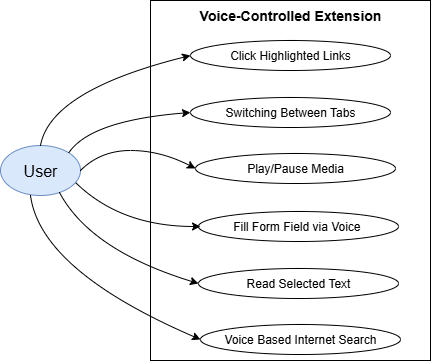
\includegraphics[width=4in]{latex/Chap3/User-Cases-Diagram.png}
   \caption{User-cases diagram of voice controlled system}
   \label{fig:usr-cases-diagram}
\end{figure}

Figure 3.3 illustrates the different ways the user interacts with the extension, including search, media control, form filling, navigation, and text-to-speech reading.

\subsection{Data Organization and Relationships}
Voice input, commands, actions, preference, language are organized follows a structured model in a way that it links natural voice input with the executable commands in action. For example “search python tutorials for beginners” is spoken by user, the raw speech is handled and recognized by web speech API influenced by language, then appropriate commands is matched and maps to the Search Handler with the site to visit and query.

 \begin{figure}[H] 
   \centering
   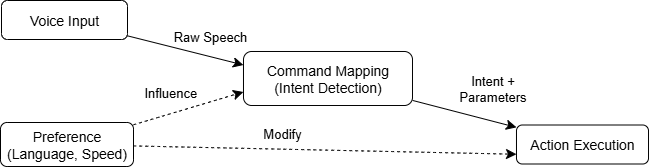
\includegraphics[width=6in]{latex/Chap3/Data-relationship.png}
   \caption{Data Relationship Diagram Among Components}
   \label{fig:model}
\end{figure}

Figure 3.4: Data Structure and Relationships illustrates how commands, actions, and user preferences are organized in the system. Spoken input is first recognized and mapped into intents with associated parameters. User Preferences such as language, zoom level, reading speed modify both interpretation and execution. Finally mapped commands are executed as system action to interact with browser.

\bigskip
\bigskip
\bigskip

\section{Demonstration and Illustration}
The extension’s usability is demonstrated through:

\begin{figure}[ht]
   \centering
   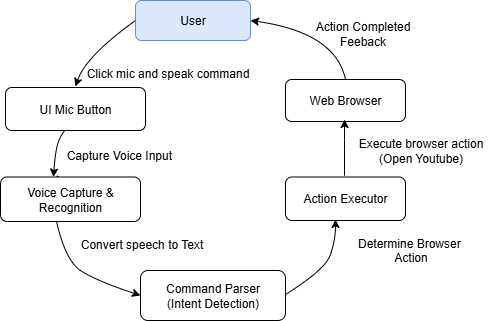
\includegraphics[width=5.5in]{latex/Chap3/sequence-diagram.png}
   \caption{Sequence diagram with detailed workflow }
   \label{fig:model}
\end{figure}
Figure 3.5: sequence diagram presents the detailed step-by-step message flow between elements for single command execution.

\begin{itemize}
\item The process initiates while user click on mic and speak any command.
\item	UI mic button captures the voice input and pass through it to the Voice Capture \& Recognition component.
\item This component converts speech into text and transfer it to the Command Parser.
\item Command Parser detect the intent by parsing the text and transfer appropriate browser action to the action executor section. 
\item Action Executor Component executes the browser action in web browser such as inline search in YouTube shown in above figure. 
\item Web browser then send the feedback to the user by displaying the output.
\end{itemize}

\section{Algorithmic Approach For Implementing Features}
In this section, different feature modules are described along with algorithms which show how each feature can be implemented. The implementation process with code is discussed in Chapter 4 for each feature.

\subsection{Capturing and Interpreting Voice Commands}
This subsection describes how to capture and interpret voice commands spoken by users. \texttt{Algorithm 1} describes the way of  processing of a voice command from capture to execution. Speech Recognition API is used here to detect text from speech. If intent matches with commands, it executes actions otherwise provides error message to user.

\begin{algorithm}[H] 
    \caption{Voice Command Processing from capturing to execution}
    \label{alg:voice_command_processing}
    \textbf{Input:} voice\_input
    \textbf{Output:} executed\_action
    \begin{algorithmic}[1] % The [1] option enables line numbering
        \State Capture \Call{voice\_input}{} from microphone
        \State Convert \Call{voice\_input}{} to text using Speech Recognition API
        \State Detect language of text
        \If {intent matches known command}
            \State Execute corresponding action
        \Else
            \State Provide error/feedback to user
        \EndIf
        \State \Return executed\_action
    \end{algorithmic}
\end{algorithm}


\subsection{Media Playback and Sound Management}

This feature allows the user to control media playback (play, pause, volume, mute, forward, backward) using voice commands. \texttt{Algorithm 2} describes how intent is detected and how associated video content is manipulated in the DOM.

\begin{algorithm}[H]
    \caption{Media Playback and Sound Management}
    \label{alg:media_control}
    \textbf{Input:} voice\_command  
    \textbf{Output:} media\_state\_changed  
    \begin{algorithmic}[1]
        \State Capture voice command
        \State Convert to text and extract intent
        \If {intent = "play"} 
            \State Execute \Call{video.play}{} 
        \ElsIf {intent = "pause"} 
            \State Execute \Call{video.pause}{} 
        \ElsIf {intent = "volume up"} 
            \State Increase volume by 10\% 
        \ElsIf {intent = "volume down"} 
            \State Decrease volume by 10\% 
        \ElsIf {intent = "forward/backward"} 
            \State Adjust \Call{video.currentTime}{} by given seconds 
        \EndIf
        \State Provide feedback to user
    \end{algorithmic}
\end{algorithm}

\subsection{Tab Navigation and Switching}

This feature allows the user to manage tab navigation(open, close, or switch browser tabs) by voice commands.\texttt{Algorithm 3} refers how tab-related intent are matched and then sends a message to Chrome’s API to perform the related action.

\begin{algorithm}[H]
    \caption{Tab Navigation and Switching}
    \label{alg:tab_management}
    \textbf{Input:} voice\_command  
    \textbf{Output:} tab\_action\_executed  
    \begin{algorithmic}[1]
        \State Capture voice command
        \State Convert to text and detect tab intent
        \If {intent = "open site"} 
            \State Extract site name and call \Call{chrome.tabs.create}{url} 
        \ElsIf {intent = "close tab"} 
            \State Call \Call{chrome.tabs.remove}{currentTab} 
        \ElsIf {intent = "switch tab"} 
            \State Identify target tab and call \Call{chrome.tabs.update}{active=true} 
        \EndIf
        \State Confirm action with visual/audio feedback
    \end{algorithmic}
\end{algorithm}



\subsection{Page View Adjustment via Voice-Controlled Scrolling and Zooming}

This feature lets the user scroll or zoom in webpage with voice commands. \texttt{Algorithm 4} describes the step by step process for mapping commands to page events like window scroll or zoom adjustment.

\begin{algorithm}[H]
    \caption{Scrolling and Zooming Process}
    \label{alg:scroll_zoom}
    \textbf{Input:} voice\_command  
    \textbf{Output:} adjusted_page_view  
    \begin{algorithmic}[1]
        \State Capture voice command
        \State Convert to text and detect scroll/zoom intent
        \If {intent = "scroll up"} 
            \State Execute \Call{window.scrollBy}{} by X pixels to top
        \ElsIf {intent = "scroll down"} 
            \State Execute \Call{window.scrollBy}{} by X pixels to bottom
        \ElsIf {intent = "zoom in"} 
            \State Increase \Call{document.body.style.zoom}{} by 10\% 
        \ElsIf {intent = "zoom out"} 
            \State Decrease \Call{document.body.style.zoom}{} by 10\% 
        \EndIf
        \State Provide feedback bubble to confirm change
    \end{algorithmic}
\end{algorithm}

\subsection{Link Highlighting and Selection}

This feature allows the user to highlight, hide, or click web page links using voice commands. All visible links are numbered, and the user can refer to them by spoken numbers or partial text are described in \texttt{Algorithm 5}.

\begin{algorithm}[H]
    \caption{Link Highlighting and Selection}
    \label{alg:link_interaction}
    \textbf{Input:} voice\_command  
    \textbf{Output:} link\_highlighted/clicked  
    \begin{algorithmic}[1]
        \State Capture voice command
        \State Convert to text and detect link intent
        \If {intent = "show links"} 
            \State Highlight all links with numeric labels
        \ElsIf {intent = "hide links"} 
            \State Remove all link overlays
        \ElsIf {intent = "click link"} 
            \If {value is number} 
                \State Click link by index 
            \Else 
                \State Find link by matching title text and click 
            \EndIf
        \EndIf
        \State Provide feedback about clicked link
    \end{algorithmic}
\end{algorithm}

\vspace{1in}

\subsection{Text-to-Speech Conversion with highlighted sentence}

This feature enables the user to listen to web page text read aloud.\texttt{Algorithm 6} describes how the system detects the selected text, highlights it sentence by sentence, and uses the speech synthesis API to read it loudly.

\begin{algorithm}[H]
    \caption{Reading Selected Text Process}
    \label{alg:read_text}
    \textbf{Input:} selected\_text  
    \textbf{Output:} audio\_narration  
    \begin{algorithmic}[1]
        \State Detect if text is selected on webpage
        \If {selection is empty} 
            \State Provide error feedback 
        \Else 
            \State Pass selected text to \Call{SpeechSynthesis}{}
            \State Highlight sentence sequentially during reading
            \State Auto-scroll page along with reading
        \EndIf
    \end{algorithmic}
\end{algorithm}


\subsection{Voice Controlled Inline Search Execution }

\texttt{Algorithm 7} demonstrates how the system performs inline search without opening a new tab(Google, YouTube). At first it clears the input, insert the query, then submit the query to display the output.

\begin{algorithm}[H] 
    \caption{Inline Search}
    \label{alg:inline_search}
    \textbf{Input:} query, active\_tab
    \textbf{Output:} search\_results
    \begin{algorithmic}[1]
        \State Check if \textbf{active\_tab} supports inline search
        \State Clear current search input
        \State Insert \textbf{query} into search box
        \State Press Enter to display results
        \State Highlight first search result (optional)
    \end{algorithmic}
\end{algorithm}

\subsection{System Response Time}
In this subsection, an equation is presented to calculate the total time taken from the capture of the voice input to perform execution.
\vspace{.5in}

\begin{equation}
T_{response} = T_{capture} + T_{recognition} + T_{parsing} + T_{execution}
\end{equation}
\begin{align*}
T_{\text{Response}} &= \text{Time taken from input to execute the action.} \\
T_{\text{Capture}} &= \text{Time to capture voice input} \\
T_{\text{Recognition}} &= \text{Time for speech-to-text conversion} \\
T_{\text{Parsing}} &= \text{Time to parse command and determine intent} \\
T_{\text{Execution}} &= \text{Time to execute the browser action}
\end{align*}

\section{Scalability and Extensibility}
The modular design of this system enables to add new commands and services(like Google Doc voice typing).The design of the system makes this scalable and extensive to new features. It can support to a new language commands by adding them in new JSON file. In future it is possible to add NLP features for more natural speech interpretation and reduce response time. 
\section{Conclusion}
This chapter presents the architecture, workflow of the voice based chrome extension. This system is modular, scalable and user-friendly by enabling voice command inclusion. Algorithms and diagrams clarify the step by step system design and its workflow from user input to actions. 
This proposed methodology provides a solid foundation to design, develop and testing the system and also its future enhancement by adding new features and including new languages.










%\chapter{Simulation Results and Discussion}
\chapter{Implementation and Result Analysis}

\section{Introduction}
This chapter demonstrates the implementation and result analysis of the Voice Search Chrome Extension. This chapter describes the  technologies are used here to develop, development details with code snippet, testing strategies and performance evaluation of the system. Screenshot and tables are included to show the functionalities and performance of the project.

The primary goal of this chapter is to show how the methodology proposed in the Chapter 3 has been implemented into a working software product. The result highlights the efficiency, accuracy and usability of the extension.



\section{Technologies Used and Their Application}
Table 4.1 demonstrates each technology used here to ensure performance, modularity and accessibility.
\begin{table}[H]
\centering
\caption{Technologies Used and Their Application}
\label{tab:technologies_used}
\begin{tabular}{|p{4cm}|p{10cm}|}
\hline
\textbf{Technology} & \textbf{Purpose / How It Was Used} \\ \hline
JavaScript (ES5) & Used to implement core logic for capturing voice, parsing commands, executing browser actions \\ \hline
Chrome Extension APIs & Used for tab management, content scripts, and browser interaction \\ \hline
Web Speech API & Converts voice input to text and detects language (English/Bengali). \\ \hline
JSON & Stores commands and mappings to the corresponding actions \\ \hline
HTML / CSS & used for designing Floating mic button and UI for feedback \\ \hline

\end{tabular}
\end{table}


\section{Implementation Details and Results}

\subsection{Voice Input Process}
Voice Input Process deals with the receiving voice commands from the users and converts them into text and pass for next stage. This process is implemented in core.js. Browser SpeechRecognition API is used to capture user voice input. The speech recognition object initialized with continuous listening and interim results for speech-to-text conversion.


\begin{minted}[
  frame=single,
  framesep=5pt,
  linenos,
  autogobble
]{javascript}
recognition = new SpeechRecognition();
recognition.lang = window.selectedLanguageCode || "en-US";
recognition.continuous = true;
recognition.interimResults = true;
\end{minted}
The system reacts to different events. \textit{onstart} - used for activating mic icon provide indication that mic is under listening mode. \textit{onerror/onend} is used to stop recognition if errors or silence occur. \textit{onresult} event sends recognized text to \textit{handleRecognitionResult} function.
\begin{minted}[
  fontsize=\small,
  frame=single,
  framesep=5pt,
  linenos,
  autogobble, breaklines
]{javascript}
recognition.onstart = () => {
    document.getElementById("floating-mic").style.background = "#28a745";
    showBubble("�� Listening...");
  };

  recognition.onerror = (e) => {
    stopRecognition();
    showBubble("❌ Error: " + e.error);
  };

  recognition.onend = () => {
    document.getElementById("floating-mic").style.background = "#007bff";
  };

  recognition.onresult = handleRecognitionResult;
\end{minted}
The function \textit{handleRecognitionResult} checks transcript, match predefined command and execute corresponding browser action(e.g scroll, open site, media control). 
\begin{minted}[
  fontsize=\small,
  frame=single,
  framesep=5pt,
  linenos,
  autogobble, breaklines
]{javascript}
function handleRecognitionResult(event) {
  ......
  for (let i = event.resultIndex; i < event.results.length; i++) {
    const result = event.results[i];
    const transcript = result[0].transcript.trim().toLowerCase();
    const isFinal = result.isFinal;
    if (!transcript) continue;
    showBubble(isFinal ? "��️ " + transcript : "…" + transcript);
    const match = matchCommand(transcript);
    ......
\end{minted}
\subsubsection*{Screenshot}
\begin{figure}[htbp] 
    \centering
    \fbox{%
    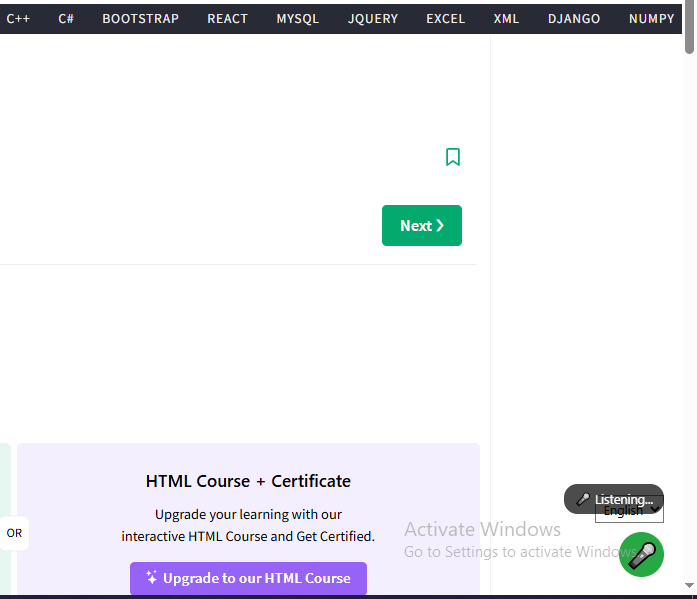
\includegraphics[width=0.7\textwidth, height=0.7\textheight, keepaspectratio]{latex/Chap4/4.3.1.listening.png}
    }
    \caption{ Active mic with “Listening...” bubble.}
    \label{fig:active_mic}
\end{figure}


\subsection{Media Control}

The Media Control module used for voice-based interaction with video element of the page. 
Once the user says \textit{``start media''}, the system enable Media Mode to allow media commands such as play, pause, volume up/down etc. 

After matching the intent, detected commands are executed on the active \texttt{<video>} element and feedback is displayed on-screen speech transcript.

\begin{minted}[fontsize=\small,
  frame=single,
  framesep=5pt,
  linenos,
  autogobble, breaklines]{javascript}
// Enabling and disabling Media Mode
if (intent === "start_media") {
   mediaMode = true;
   showBubble("Media mode enabled");
}
if (intent === "stop_media") {
   mediaMode = false;
   showBubble("Media mode disabled");
}
// Passing commands to media.js
if (mediaMode && intent.startsWith("media_")) {
   handleMediaCommand(intent, value);
}
\end{minted}

In \texttt{media.js},\texttt{handleMediaCommand()} function handle different video actions. For example, when user speak "play" video will start and when user say "pause" video will pause(shown in 2 to 10 lines). The following examples illustrate how commands are executed:

\begin{minted}[fontsize=\small,
  frame=single,
  framesep=5pt,
  linenos,
  autogobble, breaklines]{javascript}
// Playing a video
case "media_play":
   video.play();
   showBubble("Playing");
   break;
// Pausing a video
case "media_pause":
   video.pause();
   showBubble("Paused");
   break;
// Adjusting volume
case "media_volume_up":
   video.volume = Math.min(1, video.volume + 0.1);
   showBubble("Volume up");
   break;
// Other commands in similar fashion...
\end{minted}

These code snippets shows the way to map different voice commands 
to execute actions, enable consuming media content almost hands completely hands-free for users.
\subsubsection*{Screenshot}
\begin{figure}[htbp] 
    \centering
    \fbox{%
    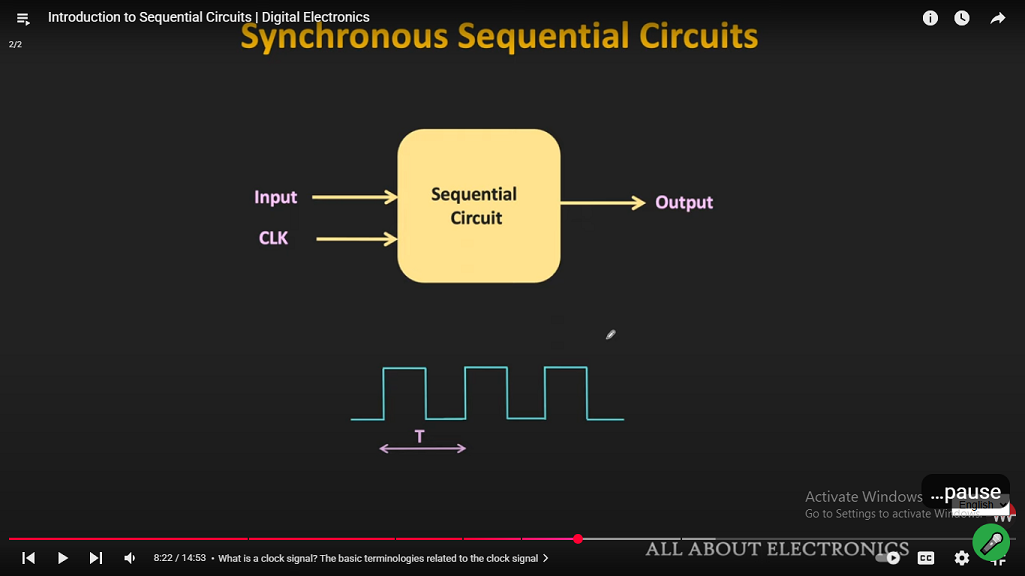
\includegraphics[width=1\textwidth, height=0.7\textheight, keepaspectratio]{latex/Chap4/4.3.2.pause.png}
    }
    \caption{ Pause the media content through voice}
    \label{fig:pause_media}
\end{figure}

\subsection{Tab Management}
This extension provides voice-controlled tab management features. It allows to users to control the browser tabs without manual interaction. It supports opening new sites of name or opening new tab, switching between tabs, view all the tabs in list of current window and closing active window through voice command. Sample examples of voice commands to access these features are given below:

\subsubsection*{Example commands:}
\begin{itemize}
    \item \texttt{"open YouTube"}: Opens \texttt{youtube.com} in a new tab.
    \item \texttt{"next tab"}: Switches to the next tab in the browser.
    \item \texttt{"previous tab"}: Switches to the previous tab.
    \item \texttt{"switch to [title]"}: Finds the title by matching the phrase after saying "switch to". 
    \item \texttt{"close tab"}: Closes the currently active tab.
    \item  \text{"show tab"}: Displays a popup window with all open tabs.
\end{itemize}

The workflow is described as user commands are recognized by the speech recognition module, then matched to intents such as \texttt{open\_site}, \texttt{tab\_next}, \texttt{tab\_previous}, or \texttt{tab\_close}.After that it sends to message to background.js file. It communicates with the Chrome Tabs API to perform the actual tab operations.

In below code describes how message is sent from core.js after matching the intent to the background.js file which executes the following tab operation.

\begin{minted}[frame=single,framesep=5pt,linenos,autogobble]{javascript}
// core.js (user says "switch to youtube")
if (intent === "tab_switch") {
  chrome.runtime.sendMessage({
    action: "switch_tab",
    query: value,   // e.g., "youtube"
  });
}
\end{minted}

\begin{minted}[frame=single,framesep=5pt,linenos,autogobble, breaklines]{javascript}
// Example: Switching to a tab by title
if (msg.action === "switch_tab") {
  const query = msg.query;
  chrome.tabs.query({ currentWindow: true }, function (tabs) {
    for (let i = 0; i < tabs.length; i++) {
      if (tabs[i].title.toLowerCase().includes(query.toLowerCase())) {
        chrome.tabs.update(tabs[i].id, { active: true });
        break;
      }
    }
  });
}
\end{minted}

This tab management module provides better accessibility to users  through the browser without manual interaction every time.

\subsubsection*{Screenshot:}
\begin{figure}[htbp] 
    \centering
    \fbox{%
    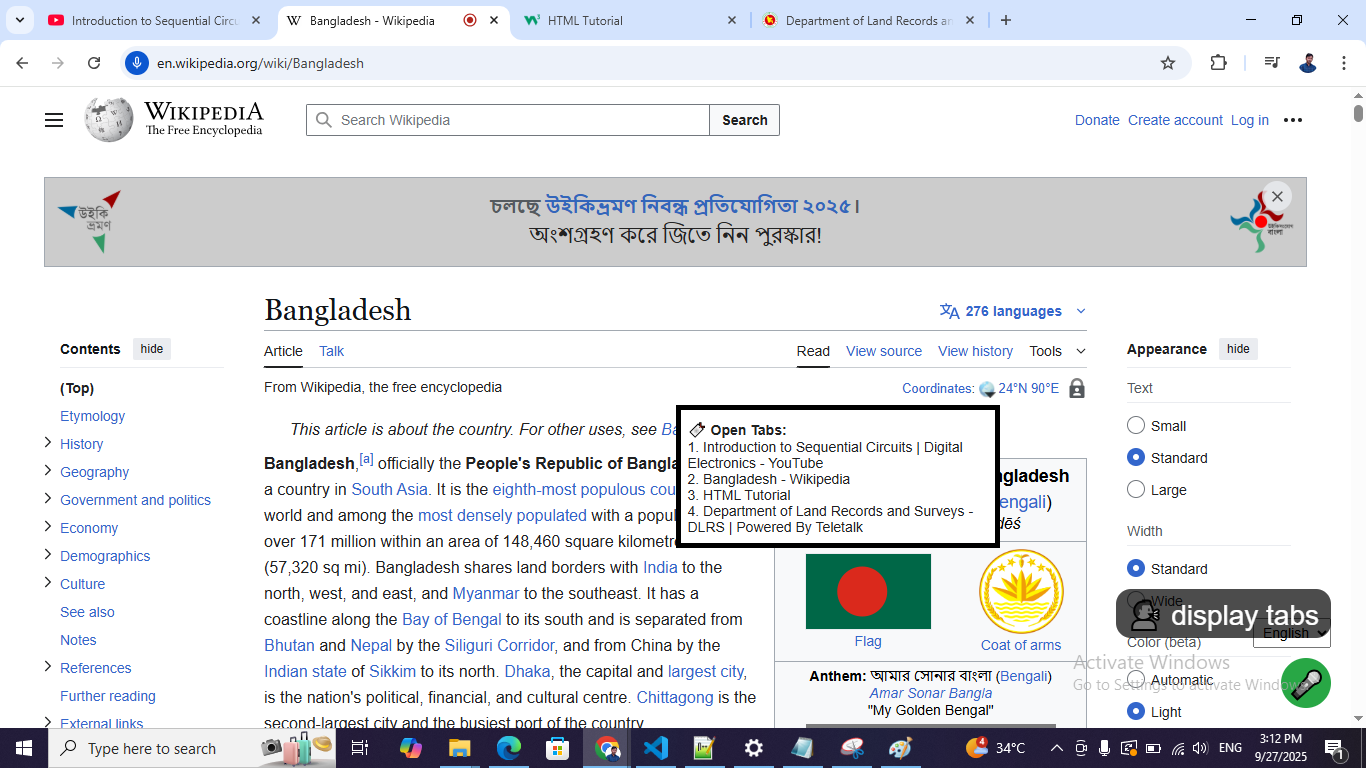
\includegraphics[width=0.7\textwidth, height=0.7\textheight, keepaspectratio]{latex/Chap4/4.3.3.tab_management.png}
    }
    \caption{ Display existing tab list of current window}
    \label{fig:display_tabs}
\end{figure}

\subsection{Scrolling and Zooming}
This feature allows users to scroll up/down the current page.Users can also set/reset zoom level through voice commands. For achieving this feature, user can perform following commands such as \texttt{scroll\_up}, \texttt{scroll\_down}, \texttt{scroll\_top}(scroll to the very top position), \texttt{scroll\_last}(scroll at the bottom of the page), \texttt{zoom\_in}, \texttt{zoom\_out}, \texttt{reset\_zoom}(to reset the zoom level to 100%). 
In below code, it shown that how "scroll up" and "zoom in" command execute those actions.

\begin{minted}[frame=single, framesep=5pt, linenos, autogobble]{javascript}
// Scroll down by 400px
if (intent === "scroll_down") window.scrollBy(0, 400);

// Zoom in by increasing current zoom step
if (intent === "zoom_in") {
    currentZoom = Math.min(currentZoom + ZOOM_STEP, 2);
    document.body.style.zoom = currentZoom;
    showBubble(`Zoomed in to ${Math.round(currentZoom * 100)}%`);
}
\end{minted}

\vspace{1in} 

\textbf{Screenshot:}

\begin{figure}[H] 
    \centering
    \fbox{%
    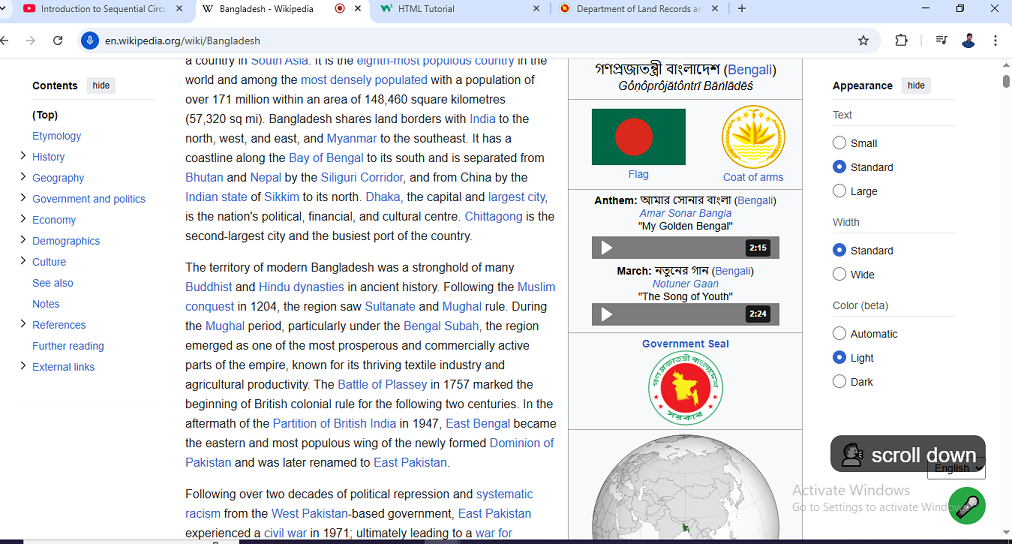
\includegraphics[width=0.8\textwidth, height=0.8\textheight, keepaspectratio]{latex/Chap4/4.3.4.scroll_down.png}
    }
    \caption{Scroll down through voice}
    \label{fig:scroll_down}
\end{figure}

\subsection{Link Interaction}
This feature enables users to highlight and click links by title on the webpage using voice commands for easier navigation. Available intents and sample commands are given below:

\begin{itemize}
    \item \texttt{show\_links}: ``show links'', ``highlight links''
    \item \texttt{click\_link}: ``click Facebook'', ``link Gmail''
    \item \texttt{hide\_links}: ``hide links'', ``remove links''
\end{itemize}

here user can click the link by saying numbers which are highlighted 
after executing \texttt{show\_links} or by saying inner text of any hyperlink.The code sample of how user can click link by title is given below:

In the below code, from 3-4 lines, it finds out the matching hyperlink from the collected hyperlink list \texttt{cachedLinks}. From 6-10, if there is any match then,it highlights the link with yellow color and click the link. Visual feedback will be provided if there is no match with title, are shown in number 11-13 lines. 

\vspace{1in}

\begin{minted}[frame=single, framesep=5pt, linenos, autogobble]{javascript}
// Find and click a link whose text contains the given title
function clickLinkByTitle(title) {
    const match = cachedLinks.find((l) =>
      l.innerText.toLowerCase().includes(title.toLowerCase())
    );
    if (match) {
        match.scrollIntoView({ behavior: "smooth", block: "center" });
        match.style.background = "yellow"; // temporary highlight
        setTimeout(() => match.click(), 600);}}
\end{minted}


% Placeholder for screenshot
\textbf{Screenshot:}

\begin{figure}[htbp] 
    \centering
    \fbox{%
    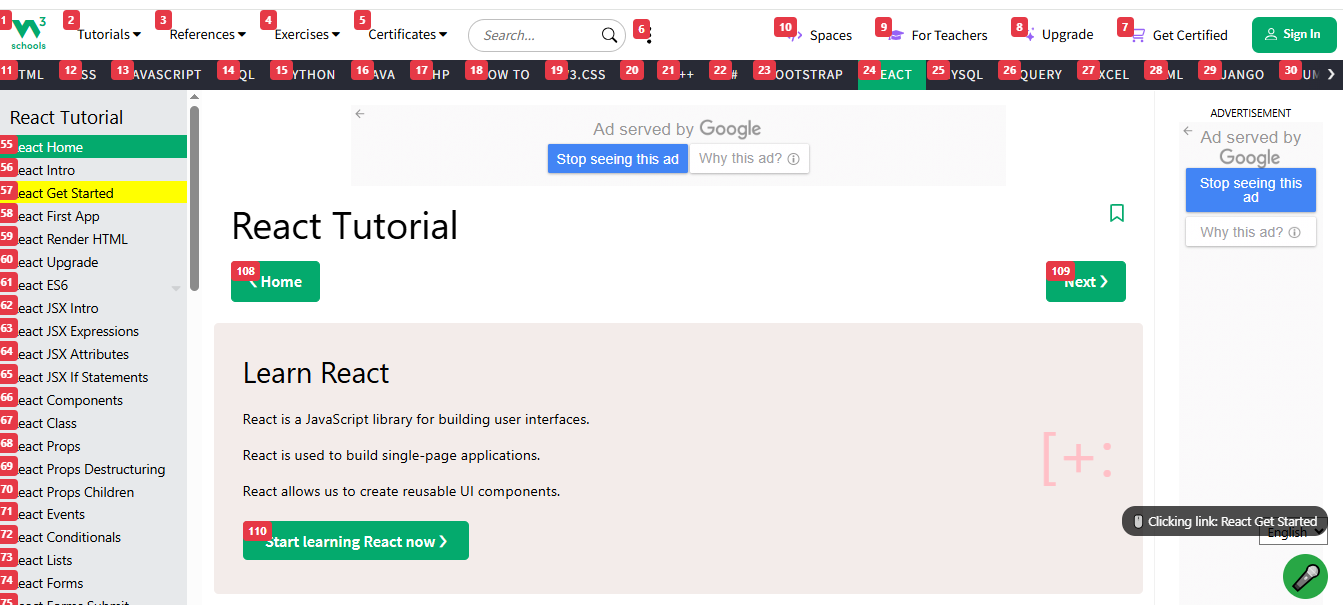
\includegraphics[width=0.8\textwidth, height=0.8\textheight, keepaspectratio]{latex/Chap4/4.3.5.highlight_links.png}
    }
    \caption{Click link by title from the highlighted links}
    \label{fig:click_highlight_links}
\end{figure}


\subsection{Reading Selected Text}
This feature is designed to improve the accessibility of extension by enabling read aloud webpage content. User can start this feature by voice command such as "start reading". Once activated, the readable sections of the webpage(paragraph, list) are highlighted through numbers.
Later, user can read those particular section by selecting the selection by number. The selected content is displayed in a dedicated pop up window and starts reading until finishing the content.
\subsubsection*{Available Commands}
\begin{itemize}
    \item \texttt{Start Reading}: User can highlight readable sections with assigns numbers.  
    \item \texttt{Read by Number [X]}: This command opens a pop up window containing the selected section by number and starts reading.
    \item \texttt{Stop Reading}: This command stops ongoing reading and closes the popup window.  
    \item \texttt{Clear Highlights}: This command is used for removing number badges from the section and borders from the page.  
\end{itemize}

\textbf{Implementation}

After triggering reading mode, \texttt{highlightReadableSections()} scans whole webpage and collect <p>, <ol> and <ul> sections.
\begin{minted}[frame=single, framesep=5pt, linenos, autogobble,breaklines]{javascript}
//
function highlightReadableSections() {
  const sections = document.querySelectorAll("p, ol, ul");
  ......
  });

  showBubble("Numbered readable sections");
}
\end{minted}

Then if user says "read number 3", then selected content is loaded by \texttt{readSectionByNumber()} 
 in pop up window starts reading the text using \texttt{startReadingSectionFromPopup} function.

\begin{minted}[frame=single, fontsize=\small, linenos]{javascript}
function readSectionByNumber(number) {
  const el = document.querySelector(`[data-read-id="${number}"]`);
  if (!el) return;
  const text = el.innerText.trim();
  showReadPopup(number, text); 
  startReadingSectionFromPopup(text); 
}
\end{minted}

\vspace{1in}

\begin{minted}[frame=single, fontsize=\small, linenos]{javascript}
function startReadingSectionFromPopup(text) {
  currentReadSentences = splitIntoSentences(text);
  currentReadSentences.forEach((s,i) => {
    const span = document.createElement("span");
    span.innerText = s + " ";
    span.dataset.index = i;
    content.appendChild(span);
  });  speakNextSentence(); }
\end{minted}


 After loading into popup window entire text is divided into sentences by function \texttt{splitIntoSentences()}.Then Browser SpeechSynthesis API reads each word sequentially by \texttt{speakNextSentence()} function. While reading each sentence is highlighted with yellow color. After finishing reading, popup window will be closed automatically.

 
\begin{minted}[frame=single, fontsize=\small, linenos]{javascript}
function speakNextSentence() {
  if (currentReadIndex >= currentReadSentences.length) return;
  const sentence = currentReadSentences[currentReadIndex];
  const u = new SpeechSynthesisUtterance(sentence);
  u.onstart = () => highlightSentence(currentReadIndex);
  u.onend   = () => { currentReadIndex++; speakNextSentence(); };
  window.speechSynthesis.speak(u);
}
\end{minted}

\subsubsection*{Screenshots:}

\begin{figure}[htbp] 
    \centering
    \fbox{%
    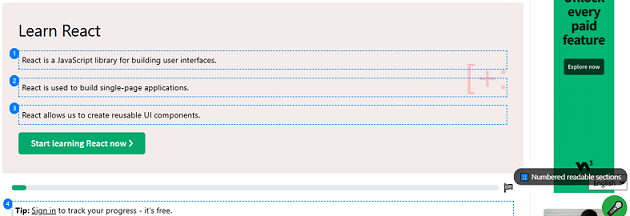
\includegraphics[width=0.8\textwidth, height=0.8\textheight, keepaspectratio]{latex/Chap4/4.3.6.1.highlight_readable_section.png}
    }
    \caption{Highlighted readable section with numeric badges}
    \label{fig:highlighted_readable_section}
\end{figure}

\begin{figure}[H] 
    \centering
    \fbox{%
    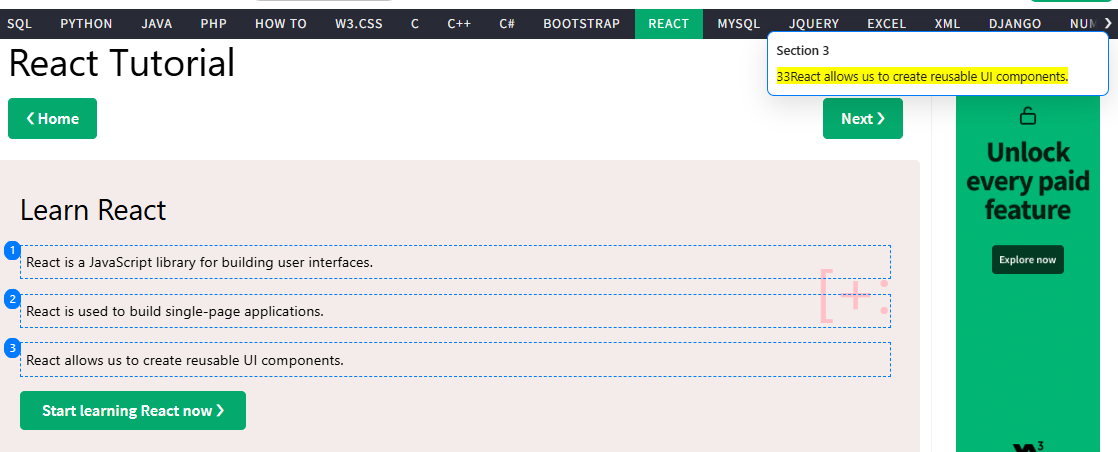
\includegraphics[width=0.8\textwidth, height=0.8\textheight, keepaspectratio]{latex/Chap4/4.3.6.2.read_from_section.png}
    }
    \caption{Read a loud from selected section in popup window}
    \label{fig:read_loud_selected_section}
\end{figure}

There is another way to implement this feature. Context menu is added here to read both English and Bengali language. User needs to select text and click context menu option from the right menu. By this way, it can read selected text loudly. Here is a screenshot of this activity.

\begin{figure}[H] 
    \centering
    \fbox{%
    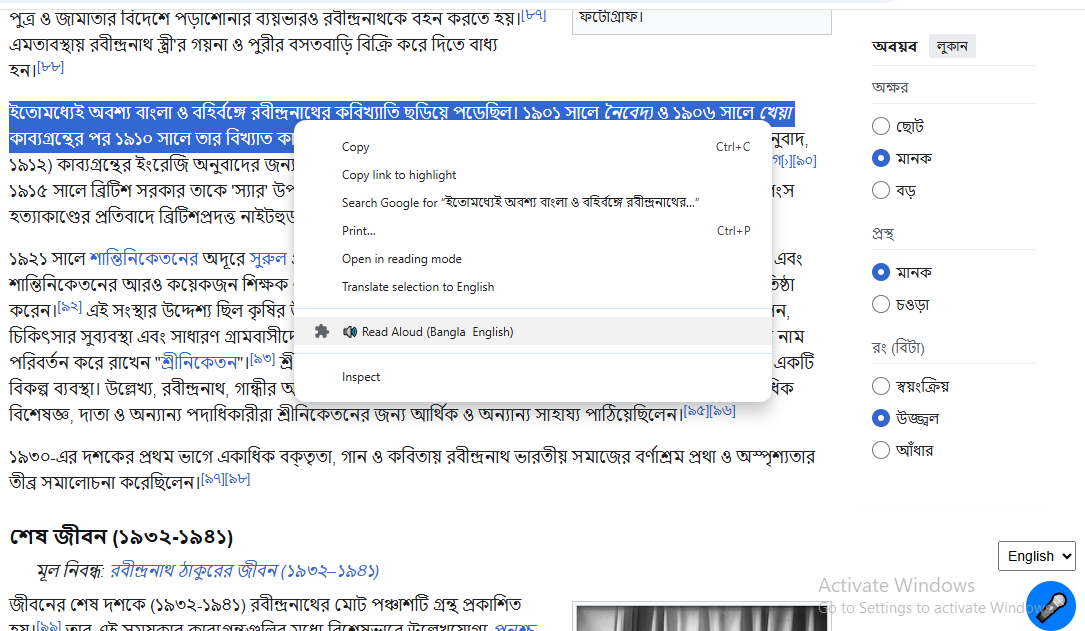
\includegraphics[width=0.8\textwidth, height=0.8\textheight, keepaspectratio]{latex/Chap4/4.3.6.3.bangla_reading.png}
    }
    \caption{Read a loud from selected Bengali text}
    \label{fig:read_loud_selected_section}
\end{figure}

\subsection{Voice-Controlled Form Fill-Up}
The Form Fill-Up feature enables user to fill the form without manual interaction, User can fill the form through voice. Right now this feature only supports English language only.

\subsubsection*{Available Commands:}

\begin{itemize}
    \item \textbf{Mode Control:} \texttt{start_form} is used to enable form mode, so that after this each commands executed for form purpose. \texttt{stop_form} is used for exit from the form mode.
    \item \textbf{Navigation:} User can use \texttt{next}, \texttt{reverse}, \texttt{back} commands to go back the previous field. User can also navigating by saying index number.
    \item \textbf{Input Handling:} Spoken words are filled into the active field; \texttt{clear} command is used to clear the active field. There is a option to fill up the password field by the secure password suggestion with \texttt{yes}/\texttt{no}. Dropdown control using \texttt{down}, \texttt{up}, or \texttt{option 3}; radio button selection can be done by saying \texttt{select male}, \texttt{choose female}.
    \item \textbf{Submission:} User can submit the form by saying \texttt{"submit form"}, \texttt{"form done"}.
\end{itemize}

\subsubsection*{System Workflow:}

The overall form handling process can be summarized as follows:
\paragraph{1. Activate Form Mode:}
When the user says \textit{``start form''}, all form fields like (\texttt{input}, \texttt{textarea}, \texttt{select}) are collected and the first field of the form is focused.

\begin{minted}[fontsize=\small,
  frame=single,
  framesep=5pt,
  linenos,
  autogobble, breaklines]{javascript}
formFields = Array.from(
    document.querySelectorAll("input, textarea, select")
).filter((el) => el.offsetParent !== null && !el.disabled);
formFields[currentFieldIndex].focus();
\end{minted}

\subsubsection*{Screenshot:}
\begin{figure}[H] 
    \centering
    \fbox{%
    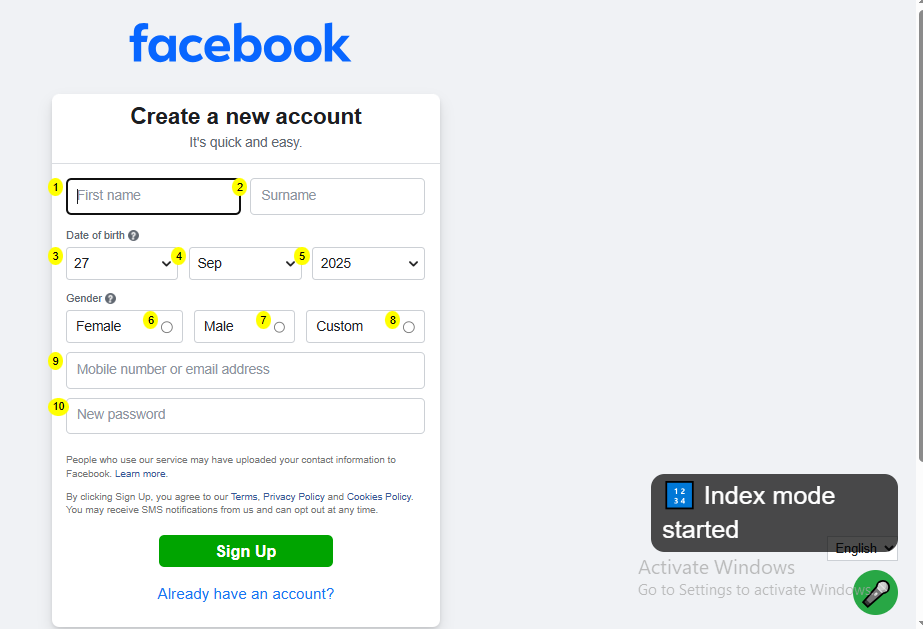
\includegraphics[width=0.7\textwidth, height=0.7\textheight, keepaspectratio]{latex/Chap4/4.3.7.form_index.png}
    }
    \caption{Start form mode with index number to each field}
    \label{fig:start_form}
\end{figure}

\paragraph{2. Navigate Between Fields:}
Users can move forward/backward in the form using \texttt{next} or \texttt{reverse}. Each navigation updates the field's current index and focuses to the new field.

\begin{minted}[fontsize=\small,
  frame=single,
  framesep=5pt,
  linenos,
  autogobble, breaklines]{javascript}
case "form_next":
  currentFieldIndex++;
  formFields[currentFieldIndex].focus();
  showBubble("➡️ Moved to next field");
\end{minted}

\paragraph{3. Input Processing:}
After second step, spoken text said by user is typed into the active field. Passwords can be filled by password suggestions and drop downs are handled by different commands.

\begin{minted}[fontsize=\small,
  frame=single,
  framesep=5pt,
  linenos,
  autogobble, breaklines]{javascript}
function handleGeneralInput(transcript, field) {
  field.value = transcript;
  showBubble("✏️ Typed: " + transcript);
}
\end{minted}

\paragraph{4. Form Submission:}
After filling up forms, if the user says \textit{``submit form''}, the system detects the form and submit the form.

\begin{minted}[fontsize=\small,
  frame=single,
  framesep=5pt,
  linenos,
  autogobble, breaklines]{javascript}
const btn = form.querySelector("button[type='submit']");
if (btn) { btn.click(); }
else { form.submit(); }
showBubble("✅ Form submitted");
\end{minted}

\subsection{Inline Search}
In this feature, user can search from google or youtube by speaking phrase. if current url is youtube, it will search in youtube otherwise the phrase term is searched in google.

When user speaks \texttt{"search some_text"}, function \texttt{isGoogleSearchPage()} or \texttt{isYouTubeSearchPage()} is called to find out the current url, later phrase is submitted by the google or youtube search bx.

\begin{minted}[fontsize=\small,
  frame=single,
  framesep=5pt,
  linenos,
  autogobble, breaklines]{javascript}
function isGoogleSearchPage() {
  return (
    location.hostname.includes("google") &&
    document.querySelector("textarea[name='q']")
  );
}

if (isGoogleSearchPage()) {
    input = document.querySelector("textarea[name='q']");
  }

  if (input) {
    input.value = query;
    input.dispatchEvent(new Event("input", { bubbles: true }));
}
\end{minted}

\subsubsection*{Screenshot:}
\begin{figure}[H] 
    \centering
    \fbox{%
    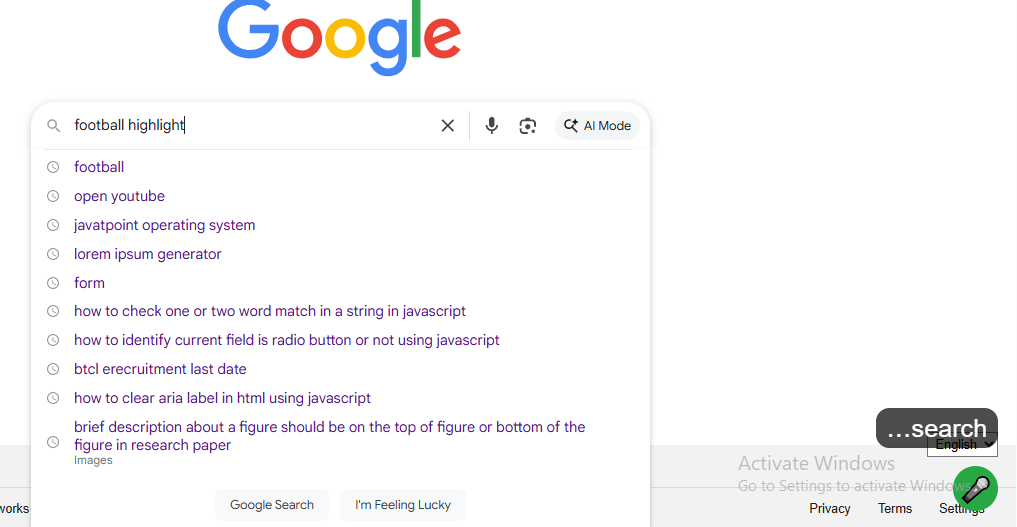
\includegraphics[width=0.7\textwidth, height=0.7\textheight, keepaspectratio]{latex/Chap4/4.3.8.inline_search.png}
    }
    \caption{Inline search in Google through voice}
    \label{fig:inline_search}
\end{figure}

\section{Testing and Result Analysis}
\begin{itemize}
\item	Functional Testing: In this test the system shows majority of the features works as expected like search commands, tab control, inline search, media control.
\item	Performance Testing: Measures response time from voice input to command action. It reflects the average time to perform any task. In this section, accuracy of the recognition and scalability are also checked. 
\item	Language Testing: In this test, checks the language is detected successfully, toggling language is worked, and voice command in both languages works just as fine majority time.
\item	Cross-page Testing: Cross functionality check is perform on different websites(Google, Youtube, Facebook etc.)
\end{itemize}


Table 4.2 shows that the test results for each feature included in extension. It detect the accuracy of the features by depicting pass/fail and response time for each item.

\begin{table}[H]
    \centering
    \caption{Feature vs. Test Result Evaluation\cite{voiceweb_test_results}}
    \label{tab:feature_test_results_professional}
    \begin{tabularx}{\textwidth}{>{\RaggedRight\arraybackslash}X c r}
        \toprule
        \textbf{Feature / Test Type} & \textbf{Status} & \textbf{Avg. Response Time (ms)} \\
        \midrule
        Voice-based Search                  & \textcolor{green!70!black}{Pass} & 350 \\ 
        Tab Control                         & \textcolor{green!70!black}{Pass} & 140 \\ 
        Form Filling                        & \textcolor{orange!80!black}{Pass (minor issue)} & 3.5 \\ 
        Media Control                     & \textcolor{green!70!black}{Pass} & 2 \\  
        Click Links by Number/title      &   
        \textcolor{green!70!black}{Pass} & 2.0 \\
        Inline Search                    &   \textcolor{green!70!black}{Pass} & 2.1 \\
        Language Toggle                     & \textcolor{green!70!black}{Pass} &  2 \\
        Cross-page Testing (Google, YouTube, Facebook) & \textcolor{green!70!black}{Pass} & 2 \\
        Recognition Accuracy                & \textcolor{blue!70!black}{80--85\% (Majority Pass)} & 1 \\
        \bottomrule
    \end{tabularx}
\end{table}


\section{Conclusion}
Chapter 4 detailed the implementation and the result analysis of the proposed system. This chapter covers both logical and physical design, technologies used, key features of the system. Also screenshots and performance and result tests confirm that the system provides responsiveness, scalability, accuracy and multilingual support. The result shows that the system is successfully translated from the proposed methodology and ready to enhance its features in future.








%Chapter{Performance Analysis}

\chapter{Conclusion and Future Works}

\section{Major Findings of the Work}
The Voice Search Chrome Extension project shows a successful implementation of a voice-controlled browser interface, enabling users to communicate with browser in English and Bangla and perform various tasks. The major findings of the work are summarized below:
\begin{itemize}
\item[1.] 	\textbf{Functional Achievement:} The proposed system successfully implemented core features: voice-based search, click highlighted links, read selected text, form filling and media control.
\item[2.]	\textbf{Multilingual Support:} Supports both English and Bangla commands, display the current language, properly identify the language and perform actions.
\item[3.]	\textbf{Real-time Performance:} Showed real time performance due to the installation on the client Chrome browser and provided smooth and real time user interaction.
\item[4.]	\textbf{Accuracy:} Achieved almost ~90 percent accuracy for English commands and ~75-80 percent accuracy for Bengali commands indicating reliable accessibility.
\item[5.]	\textbf{User-Friendly Interface:} The floating mic button provided easy access to the user to interact with the system, visual feedback improves user experience.
\item[6.]	\textbf{Modular Architecture:} The system is modular and scalable.  New commands can be easily added to the further enhancement.
\item[7.]	\textbf{Performance:} Although speech recognition module sometimes took time to take accurate input but command parsing is very fast. Overall performance is acceptable in real world.
\item[8.]	\textbf{Testing and Validation:} Functional, performance, language and cross-page testing demonstrated that the system is robust, reliable, fast and user-friendly.
\end{itemize}

\section{Future Work}
Although the current system achieved the primary objectives, there are several places to improve and enhance this system in future:
\begin{itemize}
\item[1.]	\textbf{Expand Language Support:} To add more languages apart from English and Bangla make the system widely acceptable to the wider region.
\item[2.]	\textbf{Advanced NLP:} To integrate NLP techniques to understand complex commands improving flexibility and accuracy.
\item[3.]	\textbf{Customized Commands:} This is an important feature which allow to add commands from user to make this system more user-friendly to the user and reliable. It will allow users to add custom voice commands and map them to specific actions in the browser.
\item[4.]	\textbf{Improve Accuracy:} Accuracy is one of the major problems in the speech recognition modules. So by adding noise reduction and filtering techniques, the accuracy of the speech recognition can be improved in future. 
\item[5.]	\textbf{Performance Optimization:} Reduce the latency between voice and execute action will improve the response time.
\item[6.]	\textbf{UI Enhancement:} Provide more attractive visual feedback, such as color scheme, tool tips and animations will make this system more attractive to the users.
\item[7.]	\textbf{Integration Other Features:} Summarize the content of the current page,extend support to the email, google maps, google docs or social media platforms make this system more valuable to the users.
\item[8.]    \textbf{Analytics and Usage Statistics:} Add a module to track the command uses, success rate/failure rate of the command execution help developers to optimize performance.
\item[9]	\textbf{Security and Privacy:} Enhance security by processing voice data locally will ensure user privacy.
\end{itemize}

\section{Conclusion}
The voice search chrome extension demonstrates the implementation of a successful voice controlled browser extension with dual language support and provides real-time performance, scalability and user-friendliness. The modular design and tests confirms that the proposed system is fast, reliable, secure and easy to use. The future work outlined above provides a roadmap for enhancing performance, reliability, scalability and making the system more accessible and more intelligent. 



% \label{chap:conclusion}
% 
\chapter{Conclusion and Future Works}

\section{Major Findings of the Work}
The Voice Search Chrome Extension project shows a successful implementation of a voice-controlled browser interface, enabling users to communicate with browser in English and Bangla and perform various tasks. The major findings of the work are summarized below:
\begin{itemize}
\item[1.] 	\textbf{Functional Achievement:} The proposed system successfully implemented core features: voice-based search, click highlighted links, read selected text, form filling and media control.
\item[2.]	\textbf{Multilingual Support:} Supports both English and Bangla commands, display the current language, properly identify the language and perform actions.
\item[3.]	\textbf{Real-time Performance:} Showed real time performance due to the installation on the client Chrome browser and provided smooth and real time user interaction.
\item[4.]	\textbf{Accuracy:} Achieved almost ~90 percent accuracy for English commands and ~75-80 percent accuracy for Bengali commands indicating reliable accessibility.
\item[5.]	\textbf{User-Friendly Interface:} The floating mic button provided easy access to the user to interact with the system, visual feedback improves user experience.
\item[6.]	\textbf{Modular Architecture:} The system is modular and scalable.  New commands can be easily added to the further enhancement.
\item[7.]	\textbf{Performance:} Although speech recognition module sometimes took time to take accurate input but command parsing is very fast. Overall performance is acceptable in real world.
\item[8.]	\textbf{Testing and Validation:} Functional, performance, language and cross-page testing demonstrated that the system is robust, reliable, fast and user-friendly.
\end{itemize}

\section{Future Work}
Although the current system achieved the primary objectives, there are several places to improve and enhance this system in future:
\begin{itemize}
\item[1.]	\textbf{Expand Language Support:} To add more languages apart from English and Bangla make the system widely acceptable to the wider region.
\item[2.]	\textbf{Advanced NLP:} To integrate NLP techniques to understand complex commands improving flexibility and accuracy.
\item[3.]	\textbf{Customized Commands:} This is an important feature which allow to add commands from user to make this system more user-friendly to the user and reliable. It will allow users to add custom voice commands and map them to specific actions in the browser.
\item[4.]	\textbf{Improve Accuracy:} Accuracy is one of the major problems in the speech recognition modules. So by adding noise reduction and filtering techniques, the accuracy of the speech recognition can be improved in future. 
\item[5.]	\textbf{Performance Optimization:} Reduce the latency between voice and execute action will improve the response time.
\item[6.]	\textbf{UI Enhancement:} Provide more attractive visual feedback, such as color scheme, tool tips and animations will make this system more attractive to the users.
\item[7.]	\textbf{Integration Other Features:} Summarize the content of the current page,extend support to the email, google maps, google docs or social media platforms make this system more valuable to the users.
\item[8.]    \textbf{Analytics and Usage Statistics:} Add a module to track the command uses, success rate/failure rate of the command execution help developers to optimize performance.
\item[9]	\textbf{Security and Privacy:} Enhance security by processing voice data locally will ensure user privacy.
\end{itemize}

\section{Conclusion}
The voice search chrome extension demonstrates the implementation of a successful voice controlled browser extension with dual language support and provides real-time performance, scalability and user-friendliness. The modular design and tests confirms that the proposed system is fast, reliable, secure and easy to use. The future work outlined above provides a roadmap for enhancing performance, reliability, scalability and making the system more accessible and more intelligent. 


%\startbibliography
 %\begin{singlespace} % Bibliography must be single spaced
%\bibliography{References}   % Use the BibTeX file ``References.bib''.
%\end{singlespace}
%%\setlinespacing{1.44}
\bibliographystyle{ieeetr}
%\bibliography{xbib}
% An external Abstract that can be printed at the end of the document,
% for separate submission to Rackham. Comment it out when not needed. - jg
%\startextabstractpage
%{The Title of Your Dissertation}{Your Name}{Chair: Albert Einstein}
%
		This project focuses on the development of a Chrome extension controlled by voice to improve user interactivity with web browser. Voice based browsing extensions are explored in the modern era, but most of them are limited to certain languages or do not provide flexible tab control, inline search or smooth speech interaction. The proposed solution introduces a lightweight browser extension which supports both Bangla and English commands and provides flexible features like switching between tabs, inline search for Google and Wikipedia, fill up forms, read out selected text through speech. To achieve this, we implemented speech recognition APIs, intent-based command matching and parsing for accurate result with modular Javascript arhitechture for scalability. Chrome extension APIs were integrated here for tab management, content handling and background propagation. The system was test through real browser scenerio and successfully performed site navigation, click through expected links, inline search with dual languages without noticeable lag. A special feature is added for auto silence detection and highlight-based read-0out functionality by integrating speech recognition APIs. The findings shows that the extension can help to reduce manual browsing effort by providing solutions for users with limited typing skills and handicuffs. This project shows that voice driven solution can improve web accessibility and multilingual abilities.
		
		\vspace{8pt}
		\textbf{Keywords}: Chrome extension, Speech recognition, APIs, Voice driven solution, Inline search.

	








































%\label{ExtAbstract}

%\bibliographystyle{alpha}
%\bibliographystyle{alpha}
\bibliography{bibfile}


\end{document}
